\graphicspath{{6indo-islamic/pics/},{6indo-islamic/asy/}}

\section{Indian and Islamic Mathematics}

\subsection{India, the Hindu--Arabic Numerals \& Zero}

\begin{minipage}[t]{0.65\linewidth}\vspace{-6pt}
	The Indian/South Asian subcontinent is bordered to the north by the Himalayan mountains and to the east by dense jungle. Its primary historical frontier comprised the fertile Indus valley to the west, now the central corridor of Pakistan, where recorded civilization dates to at least 2500\BC. During the first millennium \!\BC{}, Hinduism developed as an amalgamation of previous practices and beliefs; Buddhism and Jainism began to spread in the later part of this period, particularly in the Ganges valley further east.
	\smallbreak

	Alexander the Great's conquests reached the Indus in 326\BC, bringing Greek, Babylonian and Egyptian knowledge in his wake. The Greek overlords he left behind were rapidly overthrown and \phantom{the subcontinent became largely unified under the Maurya}
\end{minipage}
\hfill
\begin{minipage}[t]{0.34\linewidth}\vspace{-7pt}
	\flushright
	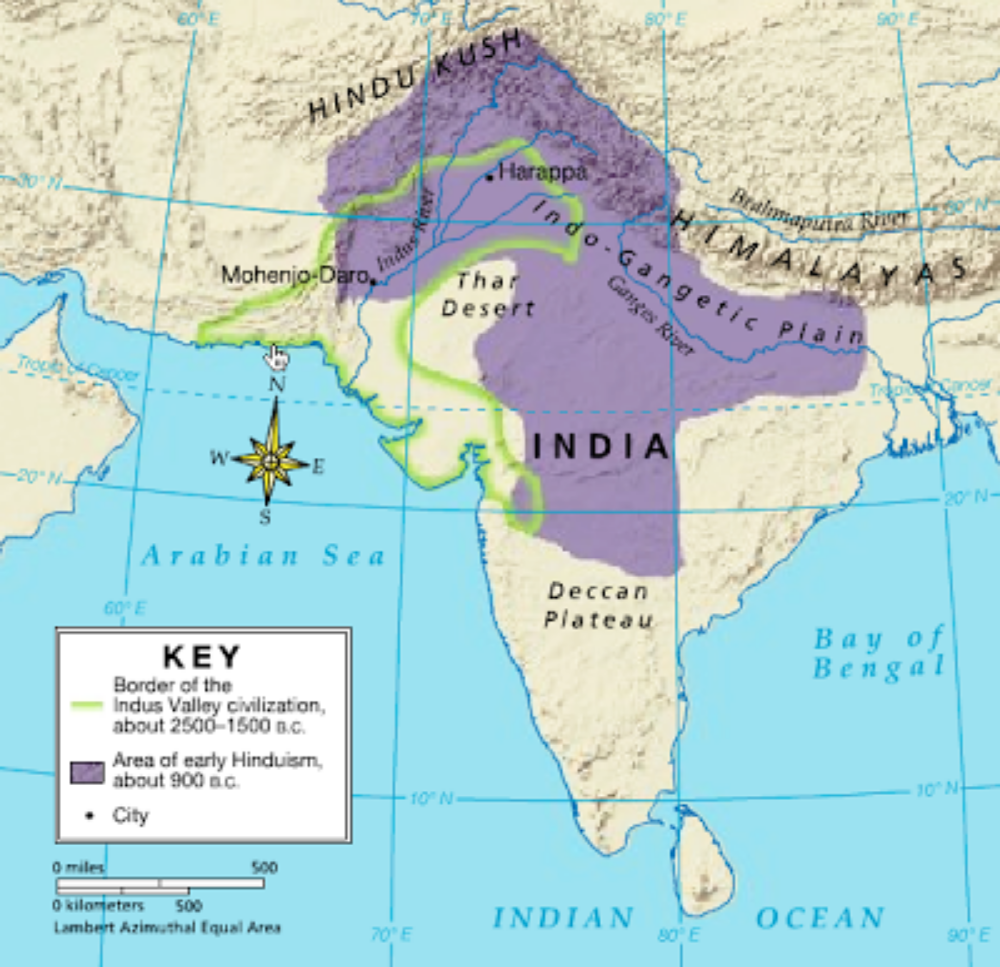
\includegraphics[scale=0.2]{Ancient_India_Map}
\end{minipage}\par
\vspace{-12pt}
the subcontinent became largely unified under the Mauryan Empire for the next 150 years. After this came 1000 years of shifting control with several invasions from the west by the Persians. Islam conquered the Indus around \AD 1000, with most of India becoming part of the Islamic Mughal Empire by the 1500s; after the Mughal decline and fragmentation, the British became dominant in 1857.
\smallbreak

The modern political situation reflects this complicated history. India gained independence from Britain in 1947 after World War II and was shortly thereafter partitioned according to religion: the greater Indus valley and the lower Ganges/Brahmaputra comprise the modern Islamic states of Pakistan and Bangladesh, with the majority of the landmass becoming the nominally secular but majority Hindu \emph{country} of India. The upper Indus valley (Kashmir) remains contested and has been the site of several military conflicts between India, Pakistan and China.
\smallbreak

Ancient India's contributions to world knowledge and development are significant; it is estimated that India accounted for 25--30\% of the world's economy during the 1\st{} millenium \!\AD\!! It was moreover a technological and cultural crossroads between East (China) and West (Greece, Persia, Rome, etc.); while some trade and knowledge passed north of the Himalayas directly between China and the Middle East/Europe, far more percolated slowly through India, being improved upon and given back in turn.


% \subsubsection*{Kharosthi numerals}
% 
% Derived from Aramaic script dating 4th--2nd C BC.
% 
% Special symbols for 10, 20.
% 
% Build to 100 additively.
% 
% 100s and larger used special symbols for powers of 10.
% 
% %Written right to left as common in West Asia.\\

\boldinline{Brahmi Numerals \& Numerical Naming}

Our primary focus is on possibly the most important practical mathematical development in history: the decimal positional system of enumeration, complete with fully-functional zero. The Brahmi numerals, one of the earliest antecedents of modern numerals, first appeared around the 3\rd{} century \BC{}.
\begin{center}
	\begin{tabular}{cccccccccc}
		1&2&3&4&5&6&7&8&9&10\\
		\IndiaBone&\IndiaBtwo&\IndiaBthree&\IndiaBfour&\IndiaBfive&\IndiaBsix&\IndiaBseven&\IndiaBeight&\IndiaBnine&\IndiaBten
	\end{tabular}
\end{center}
The example dates from around 100\BC{} and was used in Mumbai/Bombay. Additional symbols denoted multiples of 10, 100, 1000, 10000, etc. As with Chinese characters, the system was partly positional (800 would be written by prefixing the symbol for 100 by that for 8) and there was no symbol or placeholder for zero.
\goodbreak

Symbols are only part of the story. The modern approach to naming numbers and constructing large numbers can also be linked to the same period. The table below gives old Sanskrit names.
\begin{center}
	\begin{tabular}{ccccccccc}
		1&2&3&4&5&6&7&8&9\\
		eka&dvi&tri&catur&pancha&sat&sapta&asta&nava\\[0.3cm]
		10&20&30&40&50&60&70&80&90\\
		dasa&vimsati&trimsati&catvarimsat&panchasat&sasti&saptati&asiti&navati\\[0.3cm]
		100&1000&10000&100000&1000000&$10^7$&$10^8$&$10^9$&$10^{10}$\\
		sata&sahasra&ayuta&niyuta&prayuta&arbuda&nyarbuda&samudra&madhya
	\end{tabular}
\end{center}
Many European languages have Sanskrit roots; it should be no surprise that several ancient Sanskrit numbers are similar (e.g., \emph{dva} in Russian, \emph{quatre} in French). The construction of larger numbers should also seem familiar: for example \emph{tri sahasra sat sata panchasat nava} is precisely how we \emph{read} 3659.
\smallbreak
Such familiarity has its limits, for old Sanskrit verbiage doesn't map perfectly onto modern English. For instance, old Sanskrit had distinct words for powers of 10 up to (at least!) $10^{62}$, and employed a version of pre-subtraction: e.g., \emph{ekanna-niyuta} meant `one less than 100000,' or 99999.


\boldinline{Gwalior Numerals}

During the first few centuries \AD{}\!, a fully positional decimal place system came into being. The earliest evidence comes from a manuscript found in \href{http://www.bbc.com/news/uk-england-oxfordshire-41265057}{Bakhshālī} (Pakistan) in 1881, which has been carbon-dated to the 3\rd{} or 4\th{} century. The manuscript contains the earliest known version of the modern symbol for zero, a circular dot. It is conjectured that the decimal place system was inspired by the Chinese counting-board method, though convincing proof has yet to be uncovered. Regardless of attribution, Chinese mathematicians were copying the method by the 8\th{} century.\smallbreak
The examples below are better understood than the Bakhshālī manuscript and come from Gwalior (northern India) around 876.
\begin{center}
	\begin{tabular}{ccccccccccc}
		0&1&2&3&4&5&6&7&8&9&10\\
		\IndiaGzero&\IndiaGone&\IndiaGtwo&\IndiaGthree&\IndiaGfour&\IndiaGfive&\IndiaGsix&\IndiaGseven&\IndiaGeight&\IndiaGnine&\IndiaGten
	\end{tabular}
\end{center}

The similarity with modern numerals is clear;  0, 1, 2, 3, 4, 7, 9, 10 are very familiar. Zero has evolved from the Bakhshālī dot to a hollow circle. The symbols for 2 and 3 are conjectured to have developed in an attempt to write earlier versions (e.g.{} the Brahmi numerals) cursively; try writing three horizontal strokes quickly\ldots
\smallbreak
The system is fully positional. Below are the numbers 270 and 30984:
\[
	\IndiaGtwo\IndiaGseven\IndiaGzero\qquad\qquad
	\IndiaGthree\IndiaGzero\IndiaGnine\IndiaGeight\IndiaGfour
\]
Sanskrit is written left-to-right, with the leftmost digits representing the largest powers of 10. Note how zero is used as a placeholder to clarify position so that, e.g., 27, 207, and 270 are clearly distinguishable.
\goodbreak

\boldinline{Zero}
On the right is a table of modern Sanskrit names and numerals; the digits and names are certainly similar to their Gwalior counterparts.\par

\begin{minipage}[t]{0.59\linewidth}\vspace{-5pt}
	The Sanskrit \emph{shuunyá} means \emph{void} or \emph{emptiness.} It is related to \emph{svi} (hollow), which in turn derives from an ancient word meaning \emph{to grow.} This reflects a major idea within religions of the area, with the void being the source of all things, of creation and creativity. Contemplation of the void (the doctrine of Shunyata) is recommended before composing music, creating art, etc. This contrasts with the Abrahamic religions where the void is something to be feared; an early conception of hell was the eternal absence of God.
\end{minipage}
\hfill
\begin{minipage}[t]{0.4\linewidth}\vspace{-13pt}
	\flushright
	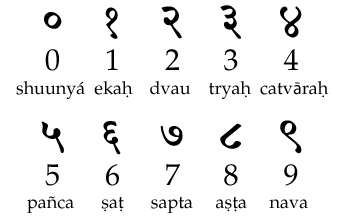
\includegraphics[scale=0.73]{sanskritnames}
\end{minipage}
\smallbreak
The Gwalior numerals travelled westwards, with Europe eventually inheriting the system via Islam; as such they are today known the \emph{Hindu--Arabic} numerals. Here is a short version of the etymological journey of zero into European languages.
\begin{itemize}
  \item \emph{Shunya} was transliterated to \emph{sifr} in Arabic where the double-meaning persisted: \emph{al-sifr} was the number zero, while \emph{safira} meant \emph{it was empty.}
  \item The term came to Europe in the 12\th{}-13\th centuries courtesy of Fibonacci where it became \emph{cifra.} This was blended with \emph{zephyrum} (\emph{west wind}/\emph{zephyr}) providing an alternate spelling.
  \item Cifra ultimately became the words \emph{cipher} (English), \emph{chiffre} (French) and \emph{ziffer} (German), meaning a figure, digit, or code.
  \item Zephyrum became \emph{zefiro} in Italian and \emph{zero} in Venetian.
\end{itemize}
Zero and the Hindu--Arabic numerals also travelled eastwards, with Qin Jiushao introducing the zero symbol into China in the 13\th{} century.
\bigbreak

Our modern understanding of zero is a fusion of several concepts:
\begin{description}
	\item[\normalfont\emph{Numerical positioning}] For instance, to distinguish 101 from 11.
	\item[\normalfont\emph{Absence of a quantity}] 101 contains no 10's.
	\item[\normalfont\emph{Symbol}] First a dot (\emph{bindu}), then a circle (\emph{chidra/randhra} meaning \emph{hole}). The relationship between \emph{shunya} and a symbol was established by \AD{2-300}, as this quote from \AD{400} (Vasavadatta) illustrates
	\begin{quote}
		The stars shone forth, like zero dots [shunya-bindu] scattered as if on a blue rug. The Creator reckoned the total with a bit of the moon for chalk.
	\end{quote}
	\item[\normalfont\emph{Mathematical operations}] By the time of Brahmagupta (7\th\,C.), a mathematical text might contain a section called \emph{shunya-gania,} with computations involving zero, including addition, multiplication, subtraction, effects on $\pm$-signs, division and the relationship with $\infty$ (\emph{ananta}). In the 12\th\,C., Bhaskaracharya stated:
	\begin{quote}
	If you were to divide by zero you would get a number that was ``as infinite as the god Vishnu.''
	\end{quote}
\end{description}


Other ancient cultures had one or more of these aspects of zero, but the Indians were the first to put them all together.
\begin{itemize}
  \item The Egyptian hieroglyph \emph{nfr} (beautiful/complete) indicated zero remainder in calculations as early as 1700\BC{} and was also used as a reference point/level in buildings.
  \item Very late in Babylonian times, a placeholder symbol was used to separate powers of 60. It was not used as a number.
  \item With the Chinese counting board, an empty space served as a placeholder.
  \item Various Mesoamerican cultures, such as the Maya, had a zero symbol that was used as a placeholder, particularly when writing dates. 
%   \item Greeks: obsessed with geometry to exclusion of other things. Not interested in number systems, saw no use for zero. Arrogant quote:
%   \begin{center}
%   Arithmetic should only be taught in democracies for it ``dealt with relations of equality''\\
%   Geometry the natural study of oligarchies, for ``it demonstrated the proportions with inequality''
%   \end{center}
\end{itemize}


\boldsubsubsection{`Real' Indian Mathematics}\phantomsection\label{pg:Mahavedi}

Indian mathematicians made great progress on several fronts, not merely the decimal place system.\par
\begin{minipage}[t]{0.56\linewidth}\vspace{0pt}
	Much ancient work was influenced by religion. For instance, the pre-Hindu \emph{sulbasutras} contained instructions for laying out altars using ruler-and-compass constructions. These could be quite complex, as the construction of the base of the \emph{Mahavedi} (great altar) shows: The center line is divided left-to-right in the ratio
	\[
		1:7:12:11:5
	\]
	and the altar contains five distinct Pythagorean triples!
\end{minipage}
\hfill
\begin{minipage}[t]{0.42\linewidth}\vspace{0pt}
	\flushright
	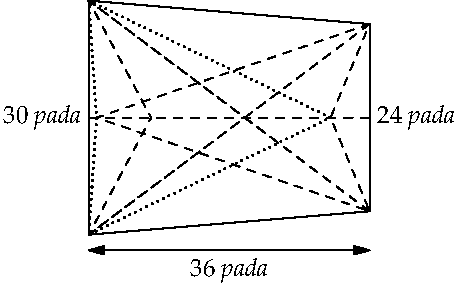
\includegraphics[scale=0.9]{india-sulba}
\end{minipage}
\medbreak

Of particular importance to our continuing narrative is Indian work on trigonometry. Here are some highlights:
\begin{itemize}
  \item The early 5\th\,C.{} text \emph{Paitāmahasiddhānta} is assumed to be an extension of Hipparchus' work, since it contains a table of chords based on a circle of radius 57,18; rather than Ptolemy's 60.
  \item Indian mathematicians instituted the use of \emph{half-chords,} in line with our modern understanding of sine. Indeed the word \emph{sine} is the result of a long sequence of (mis)translations and transliterations via Arabic and Latin from the Sanskrit \emph{jyā-ardha} (\emph{chord-half}).\footnote{
  This is also the root of the word \emph{sinus} meaning \emph{bay} or \emph{gulf} (e.g., in your nose).
 } The Indians also began to distinguish `base sine' and `perpendicular sine' (cosine).
  \item Created tables of sines/half-chords from \ang{0} to \ang{90} in steps of $\ang{3\frac 34}$, using linear interpolation to approximate values in between. By 650, Bhramagupta had much better approximations, using quadratic polynomials to interpolate. By 1530, Indian mathematicians had discovered cubic and higher approximations (essentially Taylor polynomials 130 years before Newton) for even greater accuracy of sine, cosine and arctangent.
\end{itemize}

Navigation was one of the drivers of this development. While Mediterranean sailors rarely strayed long out of sight of land, the Indians sailed the ocean and required accurate measurements to find their latitude.

\iffalse
\subsubsection*{Other Systems}

With same/similar symbols; other names. E.g. 0=shunya means ``void''\\
1 = candra (moon) or bhumi (earth)\\
2 = netra (eyes) or paska (wings of a bird), or other pairs\\
Aesthetically pleasing/literary way of counting but very hard to use: needed familiarity with particular writer's style\\

Aryabhata (b. 476) introduced alphabetical scheme, building words where each letter/sound represented a number.\\
Refined/popularized by Varurici of the Kerala school of Astronomy (same time):\\
Consonants in order represent numbers 0--9, then repeat. Vowels have no numerical value unless unpreceeded by a consonant in which case reads 0. Use vowels and available consonants to help form meaningful phrases. I.e. (from Kunjunni Raja (1963m p.123), number 1,729,133 could be said either
\begin{center}
balakalatram saukhyam: ``the company of a young woman is sheer happiness''\\
lingavyadhir asahyah: ``the demise of sexual virility is unbearable''
\end{center}

Reflects oral traditions and strict links between literacy and numeracy.





\subsubsection*{Summary}

\begin{tabular}{l p{120pt} p{150pt} p{85pt}}
Period&Main Events&Mathematics&Notable Mathematicians\\\hline
3000--1500BC&Indus Valley Civilizaton&Weights, artistic designs, brick technology&\\
1500--500BC&Aryans arrive, Hindu civilisation, records begin&Astronomy, arithmetic, Vedic geometry&Baudhayana, Apastamba, Katyayana\\
500-200BC&Rise of Buddhism and Jainism, contact with Persia. Mauryan Empire culminating in Asoka who spread Buddhism abroad&Vedic Math declines with end of ritual sacrifice. Jainia math: number theory, permutations and combinations, binomial theorem, astronomy&\\
200BC--AD 400&India divided (North, South, Punjab). Buddhism main influence on
art/sculpture&Jainia math: rules of mathematical operations, decimal place
notation, zero, algebra (simple, simultaneous, quadratic equations), square
roots, negative signs&\\
400--1200&Imperial Guptas reach height (606--647). Flowering of Indian science, philosophy, medicine, logic, grammar, literature&Bhakshali Manuscript. Aryabhaitya, etc\ldots&Aryabhata I, Varahamihira, Bhaskara I, Bhramagupta, Sridhara, Mahavira, Bhaskara II (Bhaskaracharya)\\
1200--1600&Early Muslim dynasties, Sikhism&Decline of math/learning in North. Kerala school of astronomy + math, infinite series and analysis&Narayana, Nadhava, Nilakantha
\end{tabular}

\fi

\begin{exercises}{}{}
	\exstart The \emph{Mahavedi} (pg.\,\pageref{pg:Mahavedi}) contains five Pythagorean triples; find them.
	% \begin{gather*}
	% (5,12,13),\qquad (12,16,20),\qquad (12,35,37),\\
	% (15,20,25),\qquad (15,8,17)
	% \end{gather*} 
	\begin{enumerate}\setcounter{enumi}{1}
	  \item To simplify square root expressions, Bhaskara used the formula
	  \[
	  	\sqrt{a+\sqrt b} =\sqrt{\frac 12\Big(a+\sqrt{a^2-b}\Big)} 
	  	+\sqrt{\frac 12\Big(a-\sqrt{a^2-b}\Big)}
	  \]
	  Prove Bhaskara's formula and use it to simplify $\sqrt{2+\sqrt 3}$.
	  
	  
		\item%[8-4]
	  Here is an Indian method for `finding' a circle whose area is equal to a given square.\par
	  \begin{minipage}[t]{0.62\linewidth}\vspace{-5pt}
		  In a square $ABCD$, let $M$ be the intersection of the diagonals. Draw a circle with $M$ as the center and $MA$ the radius; let $ME$ be the radius of the circle perpendicular to the side $AD$ and cutting $AD$ at $G$. Let $GN=\frac 13 GE$. Then $MN$ is the radius of the desired circle.\par
		  Show that if $AB=s$ and $MN=r$, then
		  \[
		  	\frac rs=\frac{2+\sqrt 2}6
		  \]
		  Show that this implies a value for $\pi$ equal to $3.088311755$.
	 	\end{minipage}
	 	\hfill
	 	\begin{minipage}[t]{0.35\linewidth}\vspace{-5pt}
	  	\flushright
	  	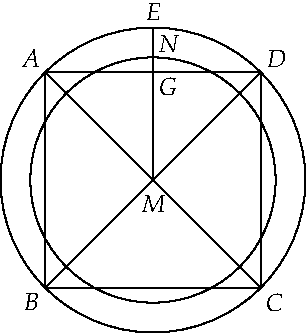
\includegraphics[scale=0.9]{india-squarecirc}
	  \end{minipage}  
	
	  
	  \item%[8-12*]
	  Solve the following problem of Mahāvīra.
	  \begin{quote}
	  	Of a collection of mango fruits, the king took 1/6; the queen took 1/5 of the remainder, and the three chief princes took 1/4, 1/3, 1/2 of what remained at each step. The youngest child took the remaining three mangoes. O you, who are clever in working miscellaneous problems on fractions, give out the measure of that collection of mangoes.
	  \end{quote}
	\end{enumerate}
\end{exercises}



\clearpage


\subsection{Islamic Mathematics I: Algebra}\label{sec:islamalgebra}

Muhammad ibn Abdullah was born in Mecca (modern Saudi Arabia) in 570. Around 610 he began preaching \emph{Islam} (\emph{submission to the will of God})---the third of the major Abrahamic religions, (chronologically) following Judaism and Christianity. After several years of exile, he returned with an army, conquering Mecca a few years before his death in 632.\smallbreak

Through military conquest, Muhammad's successors expanded the caliphate (empire) at a truly remarkable speed. At the time of his death, the \textcolor{Maroon}{Arabian peninsula} was Islamic. By 660 Islam had reached \textcolor{OrangeRed}{Libya and most of Persia,} and by 750 extended from \textcolor{Goldenrod}{Iberia \& Morocco to Afganistan \& Pakistan.} Serious schisms eventually arose\footnote{%
	In particular between the Sunni and Shia branches of the faith. Much of the modern-day tension between Saudi Arabia and Iran stems from this rupture.%
} and several successor empires emerged, the longest-lasting of which was the Ottoman Empire (c.\,1300--1922). Even though centralized political control ended long ago, Islam remains dominant in the region pictured below (with the notable exceptions of Spain and Portugal) and over a greater region of Africa and south-east Asia (e.g., Indonesia).
\begin{center}
	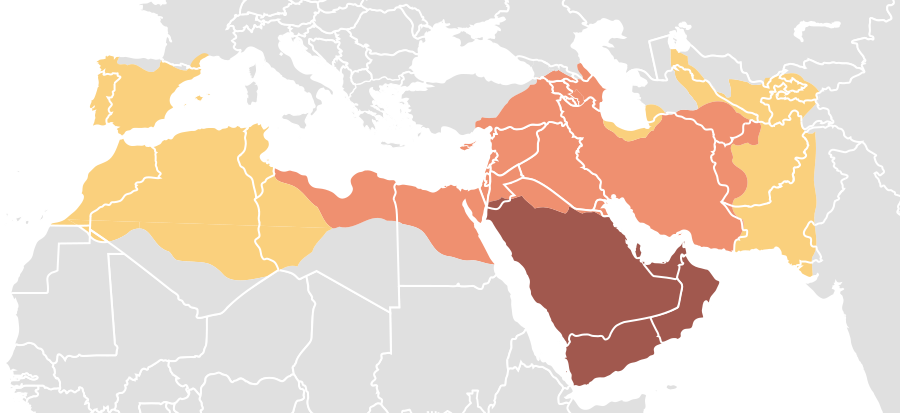
\includegraphics[width=0.7\linewidth]{caliphate.png}
\end{center}

As with the Romans, early Muslims permitted conquered peoples---including Jews and Christians (\emph{people of the book})---to maintain their culture, provided they acknowledged their overlords and paid taxes. Those who converted to Islam were welcomed as full citizens, though deconversion (apostasy) was not tolerated. Many of the great Islamic thinkers were born on the periphery and travelled to the great centers of learning, particularly Baghdad during the Islamic golden age (8\th--13\th centuries). Knowledge was also absorbed from Alexandria and western India (Pakistan). In the mid-700s paper-making came from China, greatly facilitating the dissemination and consolidation of knowledge. Schools (\emph{madrassas}) reflected a strong cultural and religious focus on learning.\smallbreak

The Islamic golden age overlapped the European \emph{dark ages} (c.\,500--1200) following the fall of Rome, during which European philosophical development stagnated. By 1200, the crusades\footnote{A series of religious--military campaigns 1096--1291 with the goal of wresting control of the Holy Land, particularly Jerusalem, from Islam.} were well underway and Islam had come to be seen as the enemy of Christian Europe. The infusion of knowledge that came to Europe from Islam around this time helped spur the European renaissance \& later scientific revolution. Among European scholars almost to the present day, it was fashionable to credit Islam merely with the \emph{preservation} of ancient `European' knowledge; a claim both fanciful and chauvinistic, but plainly stemming from medieval animosity.

\goodbreak


\boldsubsubsection{Algebra \& Algorithms}

Proof and axiomatics were learned from Greek texts such as the \emph{Elements.} Like the Greeks, Islamic scholars gave primacy to geometry and proved algebraic relations in a geometric manner.\footnote{Like Book II of the \emph{Elements.} 
Such Greek texts were venerated by Islamic scholars; recognizing the depth of Ptolemy's work on astronomy and trigonometry, they bestowed the name by which it is now known, the \emph{Almagest} (\emph{Great Work}).} Practical and accurate calculation was more important than to the Greeks, and great advances were made in this area. This included completing the development of the Indian decimal place system (hence the dual credit \emph{Hindu--Arabic} numerals).\smallbreak
The second most obvious legacy of Islamic mathematics is encountered daily in every mathematics classroom. \emph{Algebra}\footnote{Many words beginning \emph{al-} are of Arabic origin (alkali, albatross, etc.), as are others that have been latinized (elixir).} comes from the Arabic \emph{al-ğabr}, meaning \emph{restoring}. It originally referred to moving a deficient (negative) quantity from one side of an equation to another. A second term \emph{al-muqabala} (\emph{comparing}/\emph{balancing}) meant to subtract the same positive quantity from both sides of an equation.
\begin{quote}
	\begin{tabular}{l@{\quad}l}
		\emph{Al-ğabr}:&$x^2+7x=4-2x^2\implies 3x^2+7x=4$\\[4pt]
		\emph{Al-muqābala}:&$x^2+7x=4+5x\implies x^2+2x=4$
	\end{tabular}
\end{quote}
Islamic scholars did not use symbols or equations in a modern sense; statements were instead written out in sentences.


\boldinline{Muhammad ibn Mūsā al-Khwārizmī (780--850)}
	
Born near the Aral Sea in modern Uzbekistan, al-Khwārizmī eventually became chief librarian at the great school of learning, the \emph{House of Wisdom,} in Baghdad. His \emph{Compendious book on the calculation by restoring and balancing}\footnote{\emph{Al-kitāb al-mukhtasar fī hisāb al-ğabr wa’l-muqābala.}} (820) is a synthesis of Babylonian methods and Euclidean axiomatics; an algorithm demonstrated a solution, followed by a geometric proof. After being translated into Latin in the 1100s it became a standard textbook of European mathematics, displacing Euclid in places due to its greater emphasis on practical calculation. The word \emph{algorithm} reflects its importance: the Latin \emph{dixit algorismi} literally means \emph{al-Kwārizmī says.}


\begin{example*}{}{}
	Here is al-Khwārizmī's approach to the equation $x^2+4x=60$, or, more properly:
	\begin{quote}
		What must be the square which, when increased by four of its roots, amounts to sixty?
	\end{quote}
	
	\begin{minipage}[t]{0.7\linewidth}\vspace{-10pt}
		The algorithm may be applied to \emph{any} equation of the form $x^2+ax=b$ where $a,b>0$: here $a$ is the number of `roots,' and $b$ the total `amount.'
		\begin{itemize}\itemsep0pt
		  \item Halve the number of roots\hfill \big($2=\frac 12a$\big)
		  \item Multiply by itself \hfill \big($4=\frac 14a^2$\big)
		  \item Add to the total amount \hfill \big($64=\frac 14a^2+b$\big)
		  \item Take the root of this \hfill \Big($8=\sqrt{\frac 14a^2+b}$\Big)
		  \item Subtract half the number of roots \hfill \smash[t]{\Big($6=\sqrt{\frac 14a^2+b}-\frac a2$\Big)}
		\end{itemize}
	\end{minipage}
	\hfill
	\begin{minipage}[t]{0.29\linewidth}\vspace{-3pt}
		\flushright
		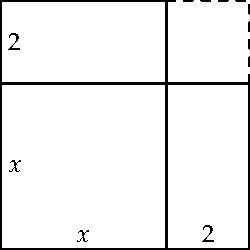
\includegraphics[scale=0.95]{islam-quad}
	\end{minipage}
	\smallbreak
	Al-Kwārizmī essentially constructs the quadratic formula $=\frac{-a+\sqrt{a^2+4b}}2$, while the pictorial justification is Euclid's (\emph{Elements}, Thm II.\,4). The geometry should be obvious: the original square ($x^2$) has been increased by four of its roots; the algorithm is simply `completing the square' $(x+2)^2=64$.
\end{example*}

Other algorithms were supplied to solve every type of quadratic.\medbreak

It is hard to notice from our example, but the crucial development from a math-history point of view is the abstraction, in a modern sense the \emph{algebra}; al-Khwārizmī's approach applies equally to numbers as it does to geometric objects, a very different approach to the geometry-focused Greeks.\medbreak

As an example of the power of this idea, consider how Abū Kāmil (Egypt 850--930) generalized Euclid's Book II geometric-algebra arguments to permit substitution, provided the resulting equation was quadratic.
\[
	\text{If }y=\frac{1+x}{3+x}\ \text{ and }\ y^2+y=1\ \text{then }x=\sqrt 5
\]
Abū Kāmil essentially substitutes $y=\frac{1+x}{3+x}$ into the quadratic (with solution $y=\frac{\sqrt 5-1}2$). While al-Khwārizmī's methods were geometrically justified, when combined in this fashion the entire process no-longer admits a straightforward geometric interpretation. This method of substitution was an early step towards establishing the modern primacy of algebra and number over geometry and length.\smallbreak
Over the following centuries, this algebraic approach was further improved. In particular, Omar Khayyam (1048--1131) produced ground-breaking work on cubic equations, astronomy, the binomial theorem, and irrational numbers.


\begin{exercises}{}{}
	\exstart %[9-4*]
	Solve the equations $\frac 12x^2+5x=28$ and $2x^2+10x=48$ using al-Khwārizmī's methods (first multiply or divide by 2).
	  
	\begin{enumerate}\setcounter{enumi}{1}
	  \item%[9-2*]
	  \label{exs:alkalgebra}
	  Al-Khwārizmī gives the following algorithm for solving the equation $bx+c=x^2$.\\
	  \begin{minipage}[t]{0.6\linewidth}\vspace{0pt}
	  \begin{itemize}\itemsep0pt
	    \item Halve the number of roots.
	    \item Multiply this by itself.
	    \item Add this square to the number.
	    \item Extract the square root.
	    \item Add this to half the roots.
	  \end{itemize}
	  Translate this into a formula. Give a geometric argument for the validity of the approach using the picture: $HC$ has length $b$ where $G$ is the midpoint; rectangle $ABRH$ has area $c$; $KHGT$ and $AMLG$ are squares; and the large square $ABDC$ has side-length $x$.
	  \end{minipage}
	  \hfill
	  \begin{minipage}[t]{0.39\linewidth}\vspace{0pt}
	  	\flushright
	  	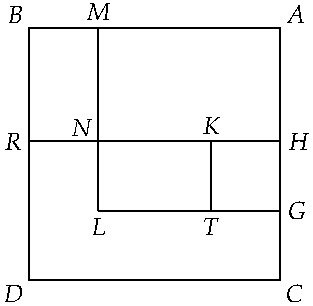
\includegraphics{hw-alk}
	  \end{minipage}
	  
	  
	  \item%[9-6]
	  Solve the following problems by Abū Kāmil (use modern algebra!).
	  \begin{itemize}
	    \item[(a)] Suppose 10 is divided into two parts and the product of one part by itself equals the product of the other part by the square root of 10. Find the parts.
	    \item[(b)] Suppose 10 is divided into two parts, each of which is divided by the other, and the sum of the quotients equals the square-root of 5. Find the parts.
	  \end{itemize}
	\end{enumerate}
\end{exercises}

\clearpage



\subsection{Islamic Mathematics II: Spherical Trigonometry and the \emph{Qibla}}

Late 8\th{} century Indian work on trigonometry, linking back to Hipparchus, was known in Baghdad, as was the work of Ptolemy. Islamic scholars were interested in trigonometry for reasons beyond mere astronomy. A primary requirement in Islam is to face the Ka'aba in the Great Mosque at Mecca when at prayer: this is the \emph{qibla} (\emph{direction} in Arabic). A mosque is typically built so that one wall faces Mecca for convenience; if not possible, an arrow indicating the \emph{qibla} might be placed in an alcove. In Muhammad's time (when Muslims faced Jerusalem not Mecca), determining the \emph{qibla} was relatively easy, though as Islam spread the curvature of the earth made determination more difficult. The religious impetus behind this problem motivated Islamic mathematics for centuries, and the methods developed (with minor modifications) are still used today, though in modern times the mathematics is very much hidden behind GPS technology!


\boldinline{Terminology and Trigonometric Tables}

Scholars worked with the Indian \emph{half-chord} (sine), and with circles of various radii. Al-Battānī (c.\,858--929) introduced an early version of \emph{cosine} as the \emph{complementary half-chord} for angles less than \ang{90}, and an analogue of the modern function \emph{versine}:\footnote{%
	\emph{Versed sine} refers to the measurement of a length in a re\emph{versed} direction (perpendicular) to that of sine.%
}
\[
	\operatorname{versin}\theta=1-\cos\theta
\]
Al-Bīrūnī (973--1048) defined versions of tangent, cotangent, secant and cosecant by projecting (e.g., a sundial) onto either a horizontal or a vertical plane. In the second picture below, the gnomon is the vertical stick of length 1. With this definition, al-Bīrūnī moves towards the modern consideration of trigonometry in terms of \emph{triangles} rather than circles.
\begin{center}
  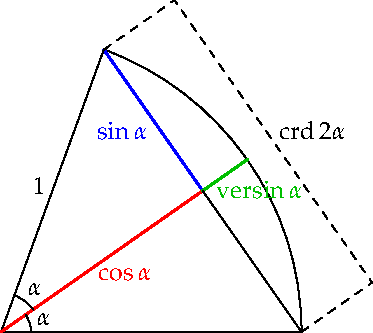
\includegraphics{islam-versin}\qquad\qquad
  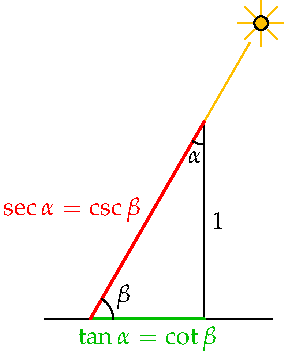
\includegraphics{islam-csc}
\end{center}\phantomsection\label{pg:sineconcave}

Trigonometric tables with improved accuracy over Ptolemy were created for all these `functions.' Abū al-Wafā (940--998) and his descendants computed sine \& tangent values for every \emph{minute} of arc accurate to \emph{five sexagesimal places} (one part in 777 million!) via repeated applications of the half-angle formula and interpolating using the downwards concavity of the sine function (draw a picture!):
\[
	\sin(\alpha+\beta)-\sin\alpha<\sin\alpha-\sin(\alpha-\beta)
	\qquad\text{whenever}\qquad
	\ang{0}<\alpha-\beta<\alpha+\beta<\ang{90}
\]

\goodbreak


\boldinline{Calculating the \emph{Qibla}}

In what follows we observe several conventions:
\begin{itemize}\itemsep0pt
  \item A single letter $A$ refers to a \emph{point} or to the \emph{angle measure} in a triangle with vertex $A$.
  \item $\arc{AB}$ means the \emph{great-circle arc} joining points $A,B$ or its \emph{arc-length.} A \emph{spherical triangle} $\triangle ABC$ comprises three points on a sphere joined by great-circle arcs.
  \item $\cl{AB}$ means the \emph{straight line} joining $A,B$ with \emph{length} $\nm{AB}$.
  \item All results are modernized and applied to a unit sphere (center $O$). The arc-length along a great-circle therefore equals the central angle subtended by that arc in radians: $\arc{AB}=\measuredangle AOB$. 3D movable versions of all pictures are online---click them! 
\end{itemize}

\begin{minipage}[t]{0.75\linewidth}\vspace{-5pt}
	Ptolemy and the Indians had already done some relevant work, though Ptolemy's approach relies heavily on Menelaus' Theorem (c.\,\AD{100}).
	
	\begin{thm*}{Menelaus}{}
		For the pictured configuration of spherical triangles on a sphere of radius 1,
		\[
			\frac{\sin\arc{CE}}{\sin\arc{AE}}=\frac{\sin\arc{CF}}{\sin\arc{DF}}\cdot\frac{\sin\arc{BD}}{\sin\arc{AB}}
		\]
	\end{thm*}
	
	Applying Menelaus is difficult since one typically needs to create many new spherical triangles. Al-Wafā simplified matters with an alternative result.
	\end{minipage}
	\hfill
	\begin{minipage}[t]{0.24\linewidth}\vspace{-5pt}
		\flushright
		\href{http://math.uci.edu/~ndonalds/math184/islam-menelaus.html}{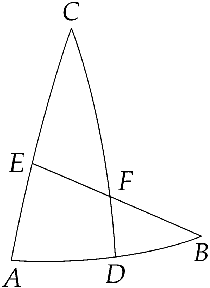
\includegraphics{islam-menelaus}}
\end{minipage}
\medbreak




\begin{thm*}{Al-Wafā}{}
	If $\triangle ABC$ and $\triangle ADE$ are spherical triangles with right angles at $B,D$ and a common acute angle at $A$, then
	\[
		\frac{\sin\arc{BC}}{\sin\arc{AC}}=\frac{\sin\arc{DE}}{\sin \arc{AE}}
	\]
\end{thm*}

In fact these ratios equal $\sin\alpha$ where $\alpha$ is the acute angle, though al-Wafā didn't say this.

\begin{proof}
	Let $O$ be the center of the sphere. Project $C$ orthogonally to the plane containing $O,A,B$ to produce $K$, then project $K$ to $\cl{OA}$ to get $L$.\par
	\begin{minipage}[t]{0.55\linewidth}\vspace{-5pt}
		Consider the right-angled \textcolor{red}{planar triangle $CKL$.} Since $\alpha$ is the angle between two planes, we have $\textcolor{red}{\alpha=\measuredangle CLK}$. Moreover
		\begin{gather*}
			\nm{CK}=\sin\measuredangle COK =\sin\measuredangle COB=\sin\arc{BC}\\
			\nm{CL}=\sin\measuredangle COL =\sin\measuredangle COA=\sin\arc{AC}
		\end{gather*}
		The usual sine formula for plane triangles says
		\[
			\sin\textcolor{red}{\alpha} =\frac{\nm{CK}}{\nm{CL}} =\frac{\sin\arc{BC}}{\sin \arc{AC}}
		\]
	\end{minipage}
	\hfill
	\begin{minipage}[t]{0.4\linewidth}\vspace{-15pt}
		\flushright
		\href{http://math.uci.edu/~ndonalds/math184/islam-alwafa.html}{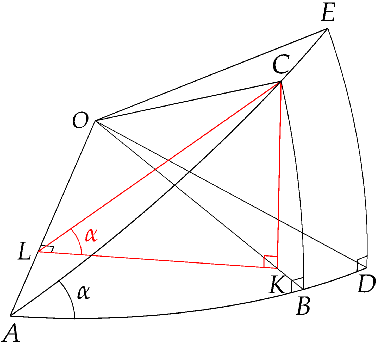
\includegraphics{islam-alwafa}}
	\end{minipage}
	\par\vspace{-3pt}
	The same ratio is obtained for $\triangle ADE$.
\end{proof}

\goodbreak

By dropping a perpendicular in a spherical triangle, Al-Wafā's result quickly yields the spherical sine rule. For the pictured triangle, drop the perpendicular to $H\in\arc{AB}$ from $C$. Al-Wafā says\par
\begin{minipage}[t]{0.65\linewidth}\vspace{0pt}
	\[
		\sin B=\frac{\sin h}{\sin a}
		\quad\text{and}\quad 
		\sin A=\frac{\sin h}{\sin b}
	\]
	By equating the $\sin h$ terms and permuting symmetrically, we've proved:

	\begin{cor*}{Sine rule}{}
		If $a,b,c$ are the side-lengths of a spherical triangle with angles $A,B,C$, then
		\[
			\frac{\sin a}{\sin A}=\frac{\sin b}{\sin B}=\frac{\sin c}{\sin C}
		\]
	\end{cor*}
\end{minipage}
\hfill
\begin{minipage}[t]{0.34\linewidth}\vspace{0pt}
	\flushright
	\href{http://math.uci.edu/~ndonalds/math184/islam-sine.html}{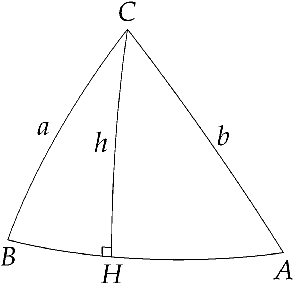
\includegraphics[scale=0.95]{islam-sine}}
\end{minipage}
\medbreak

\begin{minipage}[t]{0.65\linewidth}\vspace{2pt}
	Al-Wafā's proof was a little more complicated. He extended $\arc{AB}$ and $\arc{BC}$ to quarter-circles resulting in a spherical triangle with right-angles at $D$ and $E$. Since $\arc{DE}$ is an arc with central angle $B$, we have $\arc{DE}=B$. Since $\arc{BD}=\ang{90}$, Al-Wafā's theorem implies
	\[
		\frac{\sin h}{\sin a} =\frac{\sin B}{\sin \ang{90}}
		\implies \sin h=\sin a\sin B
	\]
	Mirroring this by extending $\arc{AB}$ past $B$ and equating the $\sin h$ terms yields the result.
\end{minipage}
\hfill
\begin{minipage}[t]{0.34\linewidth}\vspace{-10pt}
	\flushright
	\href{http://math.uci.edu/~ndonalds/math184/islam-sine2.html}{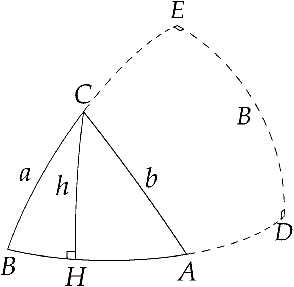
\includegraphics{islam-sine2}}
\end{minipage}
\medbreak

\begin{minipage}[t]{0.66\linewidth}\vspace{0pt}
	Using this approach, al-Wafā could solve spherical triangles and thus compute the \emph{qibla.} As with his sine rule argument, his method required several auxiliary triangles and is difficult to follow.\bigbreak
	Al-Bīrūnī further simplified matters by developing what is essentially the cosine rule. We apply his method to find the \emph{qibla} from a location $L$ (remember: our sphere (Earth!) has radius 1).\smallbreak
	Let $M$ be Mecca and $N$ the north pole. The \emph{qibla} is $\textcolor{Green}{\beta}$, the initial bearing from $L$ to $M$. Our (known) initial data are the latitudes and longitudes of $L,M$, specifically:
	\begin{itemize}\itemsep0pt
	  \item $\alpha$ is the difference in the longitudes.
	  \item $b,c$ are the \emph{colatitudes}\footnotemark{} of $M,L$ respectively. 
	\end{itemize} 
\end{minipage}
\hfill
\begin{minipage}[t]{0.32\linewidth}\vspace{0pt}
	\flushright
	\href{http://math.uci.edu/~ndonalds/math184/islam-qibla.html}{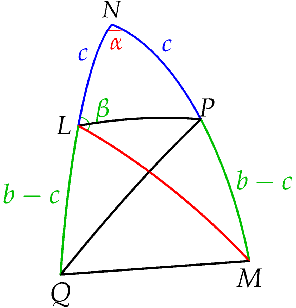
\includegraphics{islam-qibla}}
\end{minipage}
\medbreak

\footnotetext{%
	\emph{Colatitude} (equals $\ang{90}$ minus latitude) is measured southwards from the north pole. Since our model sphere has radius 1, the arc-lengths $b,c$ equal the colatitudes in radians.%
}

The cosine rule follows from Ptolemy's Theorem (pg.\,\pageref{pg:ptolemythm}). Extend $\arc{NL}$ to $Q$ with the same latitude as $M$. Similarly let $P\in \arc{NM}$ have the same latitude as $L$. By symmetry, $L,P,Q,M$ are \emph{coplanar,} whence the quadrilateral $\square LPQM$ lies on the intersection of a plane and a sphere: a circle! Measured as straight lines (chords) and using symmetry ($\nm{PQ}=\nm{LM}$ and $\nm{LQ}=\nm{PM}$), Ptolemy says
\[
	\nm{LM}\nm{PQ} =\nm{LQ}\nm{PM}+\nm{LP}\nm{QM} 
	\implies \nm{LM}^2=\nm{LQ}^2+\nm{LP}\nm{QM}
\]
\goodbreak

The great-circle arc-lengths on the sphere may be found from straight-line distances via the usual chord relations: e.g.,\par
\begin{minipage}[t]{0.67\linewidth}\vspace{-12pt}
	\def\halffrac#1{\scalebox{0.9}{$\displaystyle\frac{#1}{2}$}}
	\[
		\nm{LM}=\crd\arc{LM} =2\sin\halffrac{\textcolor{red}{\arc{LM}}}
	\]
	Ptolemy's theorem now becomes a relation between \emph{arc-lengths}
	\[
		\sin^2\halffrac{\textcolor{red}{\arc{LM}}}
		=\sin^2\frac{b-c}2 +\sin\halffrac{\arc{LP}}\sin\halffrac{\arc{QM}}
	\]
	By bisecting $\alpha$ we obtain two pairs of right-triangles; al-Wafā's theorem tells us that
	\begin{align*}
		&\sin\frac{\textcolor{red}{\alpha}}2 
		=\frac{\sin\frac{\arc{LP}}2}{\sin\textcolor{blue}{c}}
		=\frac{\sin\frac{\arc{QM}}2}{\sin\textcolor{Green}{b}}\\[3pt]
		\implies
		&\sin^2\halffrac{\textcolor{red}{\arc{LM}}}
		=\sin^2\frac{b-c}2 +\sin^2\frac{\textcolor{red}{\alpha}}2 \sin\textcolor{blue}{c} \sin\textcolor{Green}{b}\tag*{($\ast$)}
	\end{align*}
	To complete the proof we apply the multiple-angle formulæ
	\[
		\sin^2\frac x2=\frac 12(1-\cos x)\qquad
		\cos(b-c)=\cos b\cos c+\sin b\sin c
	\]

	\begin{cor*}{Cosine rule}{}
	In a spherical triangle with sides $a,b,c$ and angle $\alpha$ opposite $a$, we have
	\[
		\cos a=\cos b\cos c+\sin b\sin c\cos\alpha
	\]
	\end{cor*}
\end{minipage}
\hfill
\begin{minipage}[t]{0.32\linewidth}\vspace{0pt}
	\flushright\phantomsection\label{pg:qiblacosinerule}
	\href{http://math.uci.edu/~ndonalds/math184/islam-cosine.html}{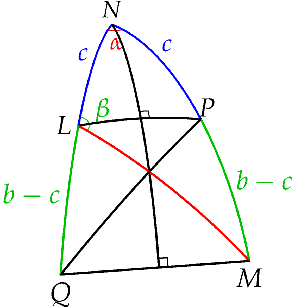
\includegraphics[scale=0.95]{islam-cosine}}
	\bigbreak
	\href{http://math.uci.edu/~ndonalds/math184/islam-cosine2.html}{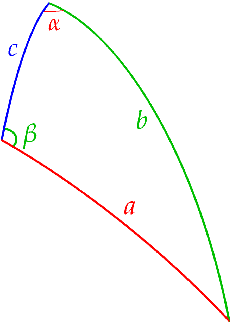
\includegraphics{islam-cosine2}}
\end{minipage}
\bigbreak

For our triangle of interest $\textcolor{red}{a=\arc{LM}}$. Given points $L,M$ (and thus $b,c,\alpha$), one uses the cosine rule to compute $a$ and then the sine rule to find the \emph{qibla} $\beta$ (whew!):
\[
	\frac{\sin \textcolor{Green}{b}}{\sin\textcolor{Green}{\beta}}
	=\frac{\sin \textcolor{red}{a}}{\sin\textcolor{red}{\alpha}} 
	\implies \sin\textcolor{Green}{\beta}
	=\frac{\sin\textcolor{red}{\alpha}\sin\textcolor{Green}{b}}{\sin \textcolor{red}{a}}
\]
\vspace{0pt}
%Whew!\bigbreak

\begin{example*}{}{}
	For fun, here is some real-world data. Mecca and London have, respectively, co-ordinates \ang{21}25'\,N, \ang{39}49'\,E and \ang{51}30'\,N, 8'\,W. This corresponds to
	\[
		\textcolor{red}{\alpha=\ang{39}57'},\qquad \textcolor{Green}{b=\ang{68}35'},\qquad \textcolor{blue}{c=\ang{38}30'}
	\]
	By al-Bīrūnī's cosine rule,
	\[
		\cos\textcolor{red}{a} =\cos \textcolor{Green}{\ang{68}35'}\cos \textcolor{blue}{\ang{38}30'}+\sin \textcolor{Green}{\ang{68}35'}\sin\textcolor{blue}{\ang{38}30'}\cos \textcolor{red}{\ang{39}57'} \implies \textcolor{red}{a=\ang{43.110}}
	\]
	Since Earth's circumference is 24900 miles, the distance London $\to$ Mecca is $\frac{43.110\times 24900}{360}=2981$ miles. Al-Wafā's sine rule computes the \emph{qibla}
	\[
		\textcolor{Green}{\beta}=\ang{180} -\sin^{-1}\frac{\sin\textcolor{red}{\alpha}\sin\textcolor{Green}{b}}{\sin \textcolor{red}{a}}=\textcolor{Green}{\ang{118}59'}
	\]
	where we subtracted from \ang{180} since the relevant angle is plainly obtuse. Check it yourself at the \href{http://www.gcmap.com/mapui?P=LON-QCA}{Great Circle Mapper} (the website uses airports for slightly different initial data).
\end{example*}


\goodbreak


\boldsubsubsection{Spherical Trigonometry Cheat Sheet}

Let $\triangle ABC$ be a spherical triangle with side-lengths $a,b,c$ on a sphere of radius 1.\medbreak

\emph{Basic trigonometry}. If $\triangle ABC$ is right-angled at $C$
\[
	\sin A=\frac{\sin a}{\sin c}\qquad \cos A=\frac{\tan b}{\tan c}\qquad \tan A=\frac{\tan a}{\sin b}
\]
Al-Wafā essentially proved the first; the others follow from trig identities ($\cos^2A=1-\sin^2A\ldots$)\medbreak

\emph{Sine rule} (Al-Wafā)
\[
	\frac{\sin A}{\sin a}=\frac{\sin B}{\sin b}=\frac{\sin C}{\sin c}
\]

\emph{Cosine rule} (Al-Bīrūnī)
\[
	\cos c=\cos a\cos b+\sin a\sin b\cos C
\]
The spherical Pythagorean Theorem is the special case $\cos c=\cos a\cos b$ \ ($C=\ang{90}$).\medbreak

If the sphere has radius $r$, simply divide all lengths by $r$ before applying the results; e.g.,
\[
	\sin A=\frac{\sin (a/r)}{\sin(c/r)}
\]
As $r\to\infty$, we have $\sin\frac ar\approx \frac ar$ and $\cos\frac ar\approx 1-\frac{a^2}{2r^2}$, which recover the flat (Euclidean geometry) versions of these statements.

\begin{examples*}{}{}
	\exstart On a sphere of radius 1, an equilateral triangle has side length $\frac\pi 3$. Splitting it in half creates two right-triangles with adjacent $\frac\pi 6$ and hypotenuse $\frac\pi 3$. The angles in the triangle are therefore
		\[
			\alpha=\cos^{-1}\frac{\tan\frac\pi 6}{\tan\frac\pi 3}=\cos^{-1}\frac 13\approx \ang{70.53}
		\]
		The angle sum in the triangle is $3\alpha\approx\ang{211.59}$!
		\begin{enumerate}\setcounter{enumi}{1}
			\item An airfield is at $C$ and two planes are at $A$ and $B$. The bearings and distances to the aircraft are \ang{45}, 2000 miles, and \ang{90}, 4000 miles respectively. Find the distance between the aircraft.\smallbreak
		This is just the cosine rule! We have a spherical triangle with sides 2000 and 4000 with angle \ang{45} between them. If $r=4000$ miles is Earth's radius, then
		\begin{gather*}
			\begin{aligned}
				\cos\frac cr &=\cos\frac{2000}r\cos\frac{4000}r+\sin\frac{2000}r\sin\frac{4000}r\cos\ang{45}\\
				&=\cos\frac 12\cos 1+\frac 1{\sqrt 2}\sin\frac 12\sin 1
			\end{aligned}\\
			\implies c=2833\text{ miles}
		\end{gather*}
		This is a little closer than the value (2947 miles) one would obtain from assuming a flat Earth!\smallbreak
		Modern navigators typically use a slightly different, though equivalent, approach to minimize the error inherent in estimating cosine for small values: look up the \emph{haversine formula} if you're interested.
	\end{enumerate}
\end{examples*}




\begin{exercises}{}{}
	\exstart A right-isosceles triangle on the surface of a unit sphere has equal legs of length $\frac\pi 4$. Find the length of the hypotenuse and the sum of the angles in the triangle. 
	\begin{enumerate}\setcounter{enumi}{1}
	  \item Explain the observation on page \pageref{pg:sineconcave} that
		\[
			\ang 0<\alpha-\beta<\alpha+\beta<\ang{90}
			\implies\sin(\alpha+\beta)-\sin\alpha<\sin\alpha-\sin(\alpha-\beta)
		\]
		is the downwards concavity of the sine function.
		
		\item Suppose we have a spherical triangle (sphere radius 1) as on page \pageref{pg:qiblacosinerule} with data
		\[
			c=\ang{30},\quad b=\ang{60},\quad \alpha=\ang{60}
		\]
		\begin{enumerate}
		  \item Use the cosine rule to find $a$.
		  \item Compute the remaining angles in the triangle. What do you observe about the sum of the angles $\alpha+\beta+\gamma$?
		\end{enumerate}
	
	  \item%[9-34*]
		Determine the \emph{qibla} for Rome (latitude \ang{41}53'\,N, longitude \ang{12}30'\,E).\par
		Repeat for the UCI campus (\ang{33}39'\,N, \ang{117}51'\,W).
	  
	  \begin{minipage}[t]{0.7\linewidth}\vspace{0pt}
		\item%[9-36*]
		Al-Bīrūnī devised a method for determining the radius $r$ of the earth by sighting the horizon from the top of a mountain of known height $h$. He would measure $\alpha$, the angle of depression from the horizontal to which one sights the apparent horizon. Show that
	  \[
	  	r=\frac{h\cos\alpha}{1-\cos\alpha}
	  \]
	  In a particular case, al-Bīrūnī measures $\alpha=34'$ from a mountain of height $652;3,18$ cubits. Assuming that a cubit equals $18''$, convert your answer to miles and compare with the modern value. Discuss the efficacy of this method.
	  \end{minipage}
	  \hfill
	  \begin{minipage}[t]{0.29\linewidth}\vspace{0pt}
	  	\flushright
	  	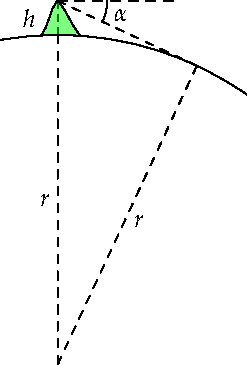
\includegraphics[scale=0.9]{hw-albiruni}
	  \end{minipage}
	  
	  
		\begin{minipage}[t]{0.7\linewidth}\vspace{0pt}
			\item On a sphere of radius $r$, Pythagoras' Theorem may be stated
			\[
				\cos\frac cr=\cos\frac ar\cos\frac br \tag{$\ast$}
			\]
			where $c$ is the hypotenuse and $a,b$ the other side-lengths. Use the Maclaurin series $\cos x=\sum\limits_{n=0}^\infty\frac{(-1)^nx^{2n}}{(2n)!}$ to expand ($\ast$) to degree 4.\par
			Suppose $a,b$ are constant so that $c$ is a function of $r$. Prove that $\displaystyle\lim\limits_{r\to\infty}c^2=a^2+b^2$. Why does this make sense?
		\end{minipage}
		\hfill
		\begin{minipage}[t]{0.29\linewidth}\vspace{0pt}
		  \hfill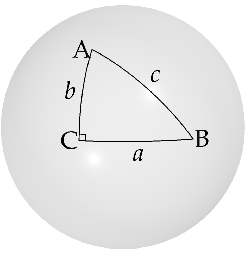
\includegraphics[scale=0.95]{spheretri3}
		\end{minipage}
  
  
  	\begin{minipage}[t]{0.7\linewidth}\vspace{0pt}
  		\item Construct a triangle on the surface of a sphere of radius $r$ by taking two lines of longitude making an angle $\theta$ from the north pole to the equator. Prove that the area of the triangle is
  		\[
  			A=r^2\theta
  		\]
  		What does Pythagoras ($\ast$) say for this triangle?\par
  		(\emph{Hint: What fraction of the sphere is covered by the triangle?})
  	\end{minipage}
  	\hfill
  	\begin{minipage}[t]{0.29\linewidth}\vspace{0pt}
  		\hfill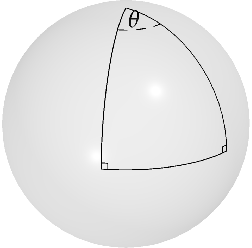
\includegraphics[scale=0.95]{spheretri}
  	\end{minipage}
	  
	\end{enumerate}
\end{exercises}